\section{Hardware choice} \label{Hardwarechoice}
From the Requirements (see \secref{Requirements}), the hardware components are chosen for the prototype. The hardware components on the vehicle (the servo for steering and the hall sensor for velocity measurement) is already chosen and will not include in this section. Beside the requirements for each components, there is considered the availability of the component and the implementation of the component in the system. 

%%%%%%%%%%%%%%%%%%%%%%%%%%%%%%%%%%%%%%%%%%%%%%%%%%%%%

\subsection{Microcontroller}
The microcontroller is the brain of the system. The purpose of the controller is to connect all the other hardware component, contain the software script of the system and control the rest of the system, with help of signals, controlled by the script.

The requirements for the microcontroller are:
\begin{itemize}
\item Have a CPU, that have a frequency greater than XX. \todo{Number}
\item Having I/O connections, both digital and analogue.
\item Having 5 free timers, to control different part of the system parallel with each other.
\item Having output connections, that can transmit PWM signals.
\item Can be powered by an external power source.
\end{itemize} 

\subsubsection{Arduino Mega 2560}
The Arduino Mega 2560 is a 8-bit microcontroller (See \figref{ArdGenMega}), which is a bigger version of the standard Arduino Uno. 

\begin{figure}[H]
	\centering
	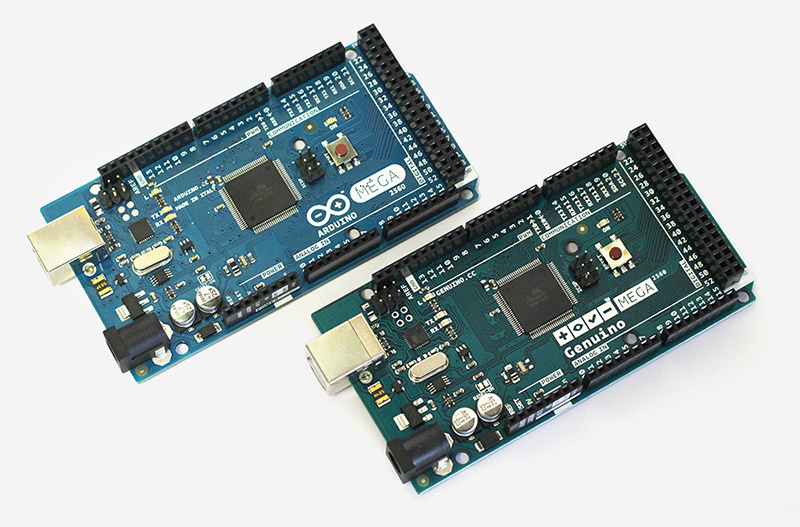
\includegraphics[width=0.60\textwidth]{figures/ArdGenMega}
		\caption{A Arduino/Genuino Mega 2560} 
	\label{ArdGenMega}
\end{figure}

It have 54 digital ports, where 15 of them can be used to PWM signals, which run all run at logic 5 volts. It have 6 timers and the CPU runs at 16 megahertz. One of the timers, do the Arduino use it self. There to also 4 UART, used to serial communication and a I2C bus. The Arduino can be powered though a USB cable or with a external power source

The Arduino Mega board will be used in this project. It have the connections to set up the already chosen hardware and have many different type of connections to set up the other hardware components. The Arduino is programmable through the Arduino software, which is writing in a slightly different type of C. The Arduino can take C and C++ files, which will making libraries and implementing them easy. 


With the choice of using a Arduino Mega, the rest of the hardware components have to have a connection possibility with it, as the Arduino will be used as the master of the system. 

%https://www.arduino.cc/en/Main/ArduinoBoardMega2560

%%%%%%%%%%%%%%%%%%%%%%%%%%%%%%%%%%%%%%%%%%%%%%%%%%%%%

\subsection{Storage}
The storage is used for saving the edge map and the route for the vehicle. This data have to be saved from use to use of the vehicle. 

The requirements for the storage are:
\begin{itemize}
\item Have to be controlled by the microcontroller.
\item The data shall be retrievable, after a power cut to the storage.
\item Have a storage of XX bytes. \todo{Number}
\item The transfer speed is greater than XX bytes per second. \todo{Number}
\end{itemize}

\subsubsection{SD card} \label{SDcard}
Secure Data card (SD card) is a non-volatile memory card. This give it the feature that the data will not be lost at a power cut off. 

It comes in various storage sizes, from 1 GB to 2 TB, depending which type of SD card it is. There is 3 types of SD card, the standard capacity (SDSC), the high capacity (SDHC) and the extended capacity (SDXC). The  difference between the different type, is the file system use on the card and the capacity cap. With the requirement of a storage size on XX bytes, the SDSC big enough with a capacity cap on 2 GB. 

The transfer speed for a SDSC card is 2 MB/s the slowest a card can maximum go by. With the requirement of a transfer speed greater than, the SDSC card is fast enough. 

To use the SDSC card, it have to setup up with 7 connections to a controller, see \figref{SDcardpinout}. The setup of the SD card is different, depended on which mode that is used. 

\begin{minipage}{\linewidth}
      \centering
      

      \begin{minipage}{0.65\linewidth}
			\begin{table} [H]
				\begin{tabular}{|l|l|l|l|}
				
				
\hline
\textbf{Pin} & \textbf{SPI}  & \textbf{One bit} 	& 	\textbf{Four bit}  \\
\hline
1			 &	Unused		 &	Unused			    &	Data 2			   \\
\hline
2			 &	Card Select	 &	Card Detection		&	Data 3			   \\
\hline
3			 &	Data in		 &	\begin{tabular}{@{}c@{}} Command \&  \\Response \end{tabular}  &	\begin{tabular}{@{}c@{}} Command \&  \\Response \end{tabular} \\
\hline
4			 &	Power		 &	Power			    &	Power			   \\
\hline
5			 &	Serial clock &	Serial clock		&	Serial clock	   \\
\hline
6			 &	Ground		 &	Ground			    &	Ground			   \\
\hline
7			 &	Data out	 &	Data 0			    &	Data 0			   \\
\hline
8			 &	Unused		 &	Unused			    &	Data 1			   \\
\hline

					
					
				\end{tabular}							
			\end{table}			
      \end{minipage}
      \hspace{0.03\linewidth}
      \begin{minipage}{0.30\linewidth}
          \begin{figure}[H]
              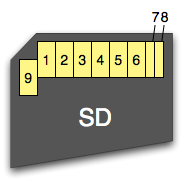
\includegraphics[width=0.95\textwidth]{figures/sdcardpinout}
              \caption{Illustration of a micro size SD card.} % http://elasticsheep.com/2010/01/reading-an-sd-card-with-an-atmega168/
              \label{SDcardpinout}
          \end{figure}
      \end{minipage}
      
  \end{minipage}
  \todo{Talk with niels about table}



The power needed for a SD card is 3.3 volts. There is three setups for the SD card: SPI, one bit and four bit. With the SPI setup, the communication between the SD card and the micro controller is on two lines. The SPI mode is the most used one for embedded systems.
With the one bit setup, the commands between the SD card and micro controller is happening on line the data is send another line. With the four bit setup, there is connected three more data lines.

In the project, the SPI setup will be used, as it is the most used method and there is not needed the extra transfer speed from the four bit setup.


A SDSC card, with a SPI setup, will be use for the project, as it have a capacity and transfer speed that meets the requirements. The data will be saved, if the power is cut off. The last requirement, the connections to the microcontroller, is possible, because the Arduino Mega 2560 controller contains  digital I/O pins, that can be use for the SPI setup for the SD card.

%https://www.sdcard.org/developers/overview/capacity/index.html
%https://www.sdcard.org/developers/overview/speed_class/
%%%%%%%%%%%%%%%%%%%%%%%%%%%%%%%%%%%%%%%%%%%%%%%%%%%%%

\subsection{Motor Driver}
The motor driver is the connection between the microcontroller, the power supply and the motor. The component is used, to separate the low power components, i.e. the microcontroller, and the high power components, i.e. the motor.

The requirements for the motor driver are:
\begin{itemize}
\item Have to be controlled by the microcontroller.
\item Can be powered by an external power source.
\item Can handle up to 7.2 volts.
\item Can power the motor in both direction.
\end{itemize}

\subsubsection{Pololu Dual VNH5019}
The Pololu dual VHN5019 motor driver shield (see \figref{MotorDrive}) is special design to Arduino boards. It can be placed directly atop of the the Arduino, where the pin will connect to the right pins on the Arduino. 

\begin{figure}[H]
	\centering
	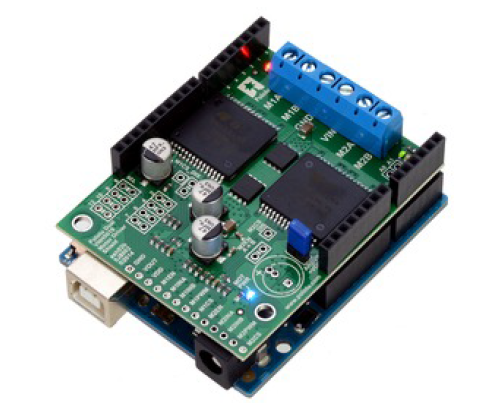
\includegraphics[width=0.50\textwidth]{figures/Motordriver}
		\caption{The motor shield atop of a Arduino Uno.} 
	\label{MotorDrive}
\end{figure}

With the motor shield, it is possible to power the Arduino from a external power source, which also deliver the power to the motor. It is also possible to have the motor shield and the Arduino powered separately. This is determined by a jumper setting on the shield, see \figref{MotorDriveIO}. The motor shield need a power voltage between 7 volts and 12 volts.

\begin{figure}[H]
	\centering
	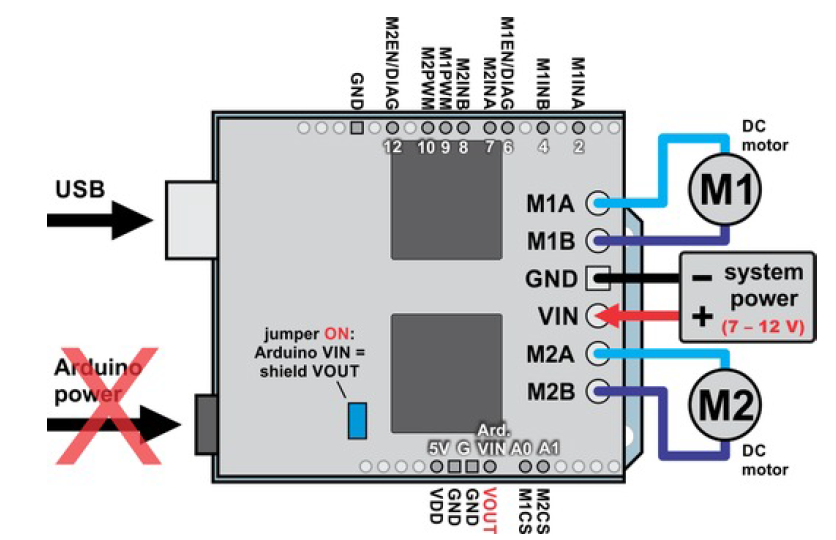
\includegraphics[width=0.60\textwidth]{figures/MotordriverIO}
		\caption{Setup for the mort shield.}
	\label{MotorDriveIO}
\end{figure}

There is two H-bridges on the board, to control two motors. As the project only have one motor, the two H-bridges will be used as one H-bridges. This will give a smaller current through the transistors in the two H-bridges and protect the system.

\begin{figure}[H]
	\centering
	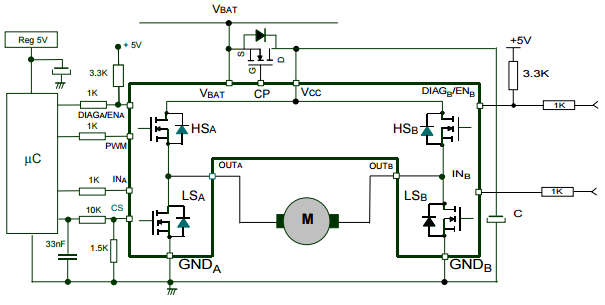
\includegraphics[width=0.85\textwidth]{figures/Hbridges}
		\caption{Illustration of the H-bridge, that the motor shield have two of.}
	\label{Hbridges}
\end{figure}.

Each of the H-bridges is controlled by a PWM signal from the Arduino. But as the H-bridges are used as one, only one will be controlled by a PWM signal. This is done by putting both H-bridges into cruise mode, one to high and the other to ground. Then the PWM signal to the H-bridge, that is set to high, will regulate the voltage sent through the motor. If the voltage have to go reverse through the motor, the settings for the two H-bridges shall swap around.

The Pololu dual VHN5019 motor driver shield will be used in this project, as it is made for the Arduino and therefore easy to implement. There to, it power the Arduino through a external power source and get a high enough power output, in each direction for the motor.

%Source: The datasheet


%%%%%%%%%%%%%%%%%%%%%%%%%%%%%%%%%%%%%%%%%%%%%%%%%%%%%

\subsection{Power Supply}
The external power supply have to both power the motor, which need a high voltage and high power and the other components, which needs low voltage and low power.

The requirements for the power supply are:
\begin{itemize}
\item Voltage output of 7.2 volts.
\item Deliverer a stable power output.
\item Can run the motor at full speed for XX. \todo{Number}
\end{itemize}

\subsubsection{Battery pack}
For the project there will be used a rechargeable battery pack on 7.2 volts. As the prototype is not set to run a long time, less than XX, a normal battery pack used for model vehicles can be used. The battery pack will deliverer a stable power output as long as the power level in the battery pack. In appendix XX \todo{Make test}, it can be seen, that the battery pack can deliverer a stable power output for XX minutes.

%%%%%%%%%%%%%%%%%%%%%%%%%%%%%%%%%%%%%%%%%%%%%%%%%%%%%

\subsection{Wireless communication}
The data from the GOT system is send to the microcontroller with this component. The transmitter will be located at the computer for the GOT system and the receiver on the vehicle. As the prototype will be tested in the control lab, the distance that the wireless communication have to send is less than 10 meters.

The requirements for the wireless communication components are:
\begin{itemize}
\item Have to be controlled by the microcontroller.
\item Have a reach greater than 10 meter. 
\item Powered by an external power supply.
\item The transfer speed is greater than XX bytes per second. \todo{Number}
\item Can be implemented in the GOT code.
\end{itemize}

\subsubsection{Xbee}
Xbee are small radio modules, that is easy to set up. Overview of the Xbee, seen on \figref{XbeeLook} and it pin layout can be seen on \figref{Xbeepinout}.


\begin{minipage}{\linewidth}
	\centering
	\begin{minipage}{0.45\linewidth}      
		\begin{figure}[H]
			\centering
			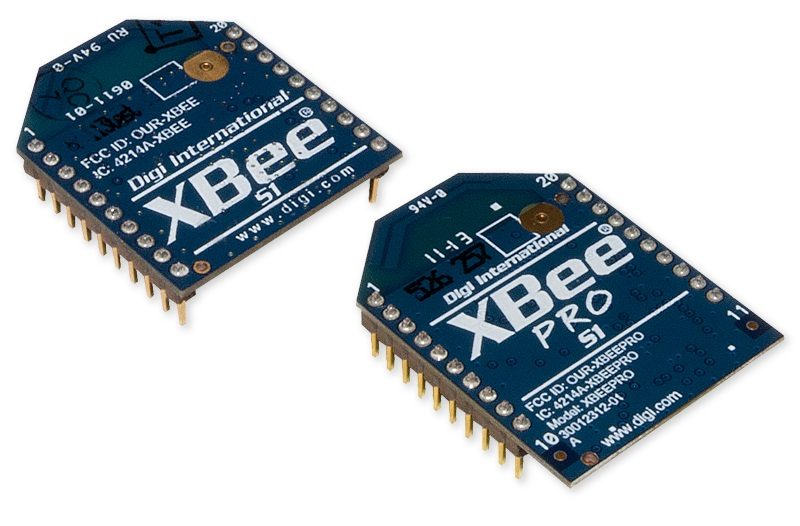
\includegraphics[width=0.95\textwidth]{figures/Xbee}
			\caption{The Xbee radio modules} 
			\label{XbeeLook}
		\end{figure}
	\end{minipage}
	\hspace{0.03\linewidth}
	\begin{minipage}{0.45\linewidth}
		\begin{figure}[H]
			\centering
			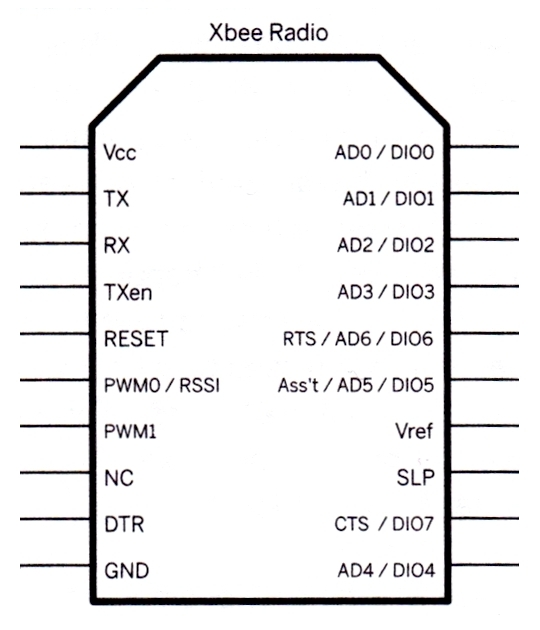
\includegraphics[width=0.95\textwidth]{figures/XbeeIO}
			\caption{Pinout for the Xbee radio modul.} 
			\label{Xbeepinout}
		\end{figure}
	\end{minipage}
\end{minipage}

\todo{Snak med vinkel om at få teksten align}

The Xbee modules communicates through a UART connection (the TX and RX pin). As the Arduino have three UART connections, beside the one use to program the Arduino with, the Xbee can be connected. The software for the GOT system is running on C\# (See in appendix \secref{GoTDescription}) and the computer running the software have some serial port, that can be connected to the software and the Xbee. So the Xbee can be used for the connection between the GOT system and the Arduino.

To run the Xbee modules, there is needed a power on 3.3 volts, a ground and a UART on 3.3 volts. The rest of the pins will not be needed in this project. It have a transfer speed up to 115.2 kilobits per second and have a reach up to 100 meters indoor and 300 meters outdoor. It transmit with 1 millivolt (0 dBm) and can receive downto -96 dBm and transmits at a 2.4 GHz frequency. The Xbee is already ready for communication, with the lower level of communication, the physical layer, already design. A transportation layer can be added to the protocol, to add more error handling and to set up how the data shall be send. \todo{Not sure if that is all the layers}

%http://www.digi.com/products/xbee-rf-solutions/modules/xbee-digimesh-2-4#specifications

%%%%%%%%%%%%%%%%%%%%%%%%%%%%%%%%%%%%%%%%%%%%%%%%%%%%%

\subsection{Angular sensor}
The angular sensor is used in the feedback for the control system.

The requirements for the angular sensor are:
\begin{itemize}
\item Have to be controlled by the microcontroller.
\item Having a sampling frequency greater than XX. \todo{Number}
\item Having a latency smaller than XX. \todo{Number}
\item Powered by an external power supply.
\end{itemize}

\subsubsection{HMC5883L}
On Sparksfun's "9 degrees of freedom" board, there is mounted a magnetometer, the HMC5883L. There will be used a magnetometer as the angular sensor, as the magnetometer can be setup as a compass and give out a angle compared to north. As the direction to north always is the same, the system will not need a new calibration of the angular sensor, if used in a new area. This will have to be needed, if the direction was taken from a local direction point, like a point in the GOT system.

\begin{figure}[H]
	\centering
	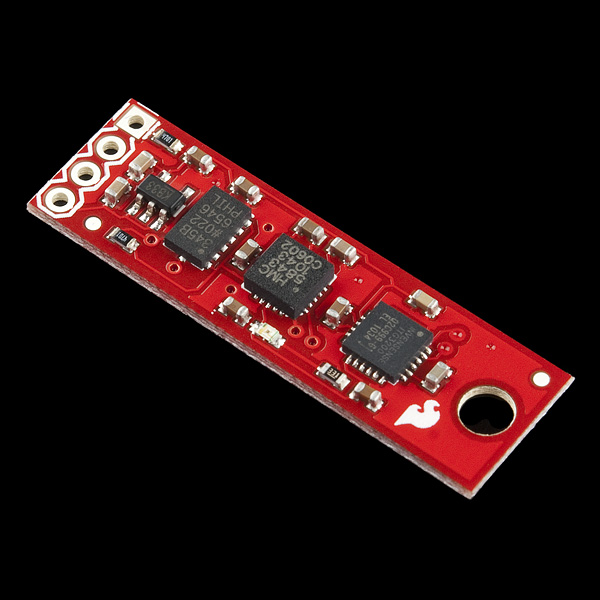
\includegraphics[width=0.50\textwidth]{figures/NineDegree}
		\caption{Sparksfun's "9 degrees of freedom" sensor stick} 
	\label{NineDegree}
\end{figure}

The "9 degrees of freedom" sensor stick, see \figref{NineDegree}, will be used in the project. Beside the magnetometer, there is a accelerometer and a gyroscope on the board, but these will not be used. The "9 degrees of freedom" sensor stick is madded to be used with a micro controller and comes with software to Arduino. It needs a I2C bus to communicated with the Arduino, which the Arduino have one of, which it not in use.


From the requirements for the system to the hardware parts, these components have been chosen. After have chosen the different hardware components for the prototype, the different components have to be implemented in the system.
%%%%%%%%%%%%%%%%%%%%%%%%%%%%%%%%%%%%%%%%%%%%%%%%%%%%%

%Note: Missing a tail.

%Pins on the arduino
%SD card (4 I/O)
%Xbee (1 TX and 1 RX)
%Hall (2 I/O)
%Angular (1 SDL and 1 SDA)
%Servo (1 PWM)
%Motor (1 PWM)
